\documentclass{class}
\usepackage[utf8]{inputenc}
%% Dependencies
% Appendices
\usepackage[toc]{appendix}
% Flexible bibliography
%\usepackage[round,authoryear]{natbib}
% ToDo notes
\usepackage{todonotes}
% Enumeration
\usepackage{nth}
% Fancy tables
\usepackage{tabularx}
\usepackage{booktabs}
% Floats
\usepackage{float}
% Numbers
\usepackage{numprint}
\npthousandsep{\,}
% Subfigures
\usepackage{subcaption}
% Correct single quotes
\usepackage{textcomp}
% Colored boxes
\usepackage{tcolorbox}
\usepackage{float}
% Custom list spacing
\usepackage{enumitem}
%colours in table 
\usepackage{multirow}
%rows in tables stretching multiple row lengths
\usepackage{nomencl}
\usepackage{amssymb}
\usepackage{siunitx}
\usepackage{pgfgantt}
\usepackage{colortbl}
\usepackage{lscape}
\usepackage{tikz}
\usepackage{rotating}
\usepackage{ifthen}
\usepackage{listings}
\usepackage{etoolbox}
\usepackage{graphicx}
\usepackage{gensymb}
\usepackage{wasysym}
\usepackage{wrapfig}
\usepackage[justification=centering]{caption}
\usepackage[english]{babel}
\usepackage{verbatim}
\usepackage{blindtext}
%\usepackage{changes}
\usepackage{tabularray}
\usepackage{amsmath}
\usepackage{amsthm}
\usepackage{hyperref}
\usepackage{diagbox}

\usepackage[
backend=biber,
style=apa,
]{biblatex}

\definecolor{darkblue}{rgb}{0, 0, 0.5}

\hypersetup{
    colorlinks=true,
    linkcolor=darkblue,
    filecolor=magenta,  
    citecolor=darkblue,
    urlcolor=cyan, 
    pdftitle={Overleaf Example},
    pdfpagemode=FullScreen,
    }
% I made the variable names slightly highlighted with grey. Do you like that? yeah that makes it more similar to jupyter and more recognizable yes
% its submitted
\definecolor{codegreen}{rgb}{0,0.6,0}
\definecolor{codegray}{rgb}{0.5,0.5,0.5}
\definecolor{codepurple}{rgb}{0.58,0,0.82}
\definecolor{backcolour}{rgb}{0.95,0.95,0.92}

\lstdefinestyle{mystyle}{
    backgroundcolor=\color{backcolour},   
    commentstyle=\color{codegreen},
    keywordstyle=\color{magenta},
    numberstyle=\tiny\color{codegray},
    stringstyle=\color{codepurple},
    basicstyle=\ttfamily\footnotesize,
    breakatwhitespace=false,         
    breaklines=true,                 
    captionpos=b,                    
    keepspaces=true,                 
    numbers=left,                    
    numbersep=5pt,                  
    showspaces=false,                
    showstringspaces=false,
    showtabs=false,                  
    tabsize=2
}
\lstset{style=mystyle}

\definecolor{lightgray}{rgb}{0.95, 0.95, 0.95}
\definecolor{red}{rgb}{1, 0, 0}
\sethlcolor{lightgray}

\def\code#1{\hl{\texttt{#1}}}
% Changes the structure from chapter-section-subsection to section-subsection-subsubsection
\renewcommand{\thesection}{\arabic{section}}
\def\title#1{\gdef\@title{#1}\gdef\THETITLE{#1}}
\newcommand{\makemytitle}{\begin{center}\Large\textbf{\THETITLE}\end{center}}
\addbibresource{bibliography.bib}
% \newcommand{\O}{\mathcal{O}}

\DeclareMathOperator*{\argmax}{arg\,max}
\DeclareMathOperator*{\argmin}{arg\,min}

\makeatletter
\patchcmd{\@chapter}{\addcontentsline{toc}{chapter}{\thechapter.\ \@chapappname}}{\addcontentsline{toc}{section}{\bibname}}{}{}
\makeatother

\title{Reinforcement Learning: Project Report}
\author{Ella Kemperman, Ioana-Anastasia Orasanu, Rostyslav Redchyts, Mila van Rijsbergen}
\begin{document}
\makemytitle
\begin{center}
    \textbf{03-04-2025}\\
\end{center}

\noindent By Ella Kemperman, student number \textit{s1119890}, Ioana-Anastasia Orasanu, student number \textit{s1112418}, Rostyslav Redchyts, student number \textit{s1113227}, Mila van Rijsbergen student number \textit{s1128515}.

\section{Introduction}
Reinforcement Learning (RL) has become increasingly relevant in Machine Learning over the past decade. RL has been irreplaceable in robotics for a while, and recently, it has also contributed to the AI revolution through approaches like RLHF (Reinforcement Learning with Human Feedback). Despite its prevalence, RL is already a mature and complex field, which can be intimidating to newcomers. Hence, in this report, we look over a few simple algorithms to explain how they work and get some insight into how they differ from each other.
\\ [0.3cm]
More specifically, various RL algorithms were implemented, and their performance in a certain environment was compared. This environment was designed specifically for this project and involved an agent, also referred to as 'the cat', navigating a 2-dimensional grid while chasing a target, metaphorically referred to as 'the mouse'.
\\[0.3cm]
The environment (see \autoref{fig:environment}) is discrete, with both the agent and the mouse traversing it by making a step in one of four directions. To increase the complexity of the environment, two obstacles have been added. Firstly, special cell types were included, called 'trees', where the cat can enter, but the mouse cannot. Secondly, walls in between the cells were added, impermeable for the cat, while the mouse can go through them. 
\\[0.3cm]
The agent receives a penalty of -1 for each step that resulted in an empty cell, a reduced penalty of -0.1 for landing on a tree, and a reward of +20 for catching the mouse (regardless of the cell type). These rewards were chosen to motivate the agent to catch the mouse as quickly while also giving some space for developing halting strategies.
\\[0.3cm]
The project consists of comparing two algorithms from Dynamic Programming (DP), which include Policy Iteration and Value Iteration (discussed in \autoref{sec: dynamic programming}; a Monte-Carlo method (discussed in \autoref{sec: monte-carlo}); and three Temporal Difference (TD) algorithms (mainly discussed in \autoref{sec: temporal difference}): Sarsa, Q-Learning, and Deep Q-Learning (discussed in \autoref{app: deep q-learning}). To achieve this, the performance of the learned policies was compared as they were being refined during learning. Furthermore, the final policies and their returns are compared as well. This is done in \autoref{sec: comparison and discussion}.

\begin{figure}[H]
    \centering
    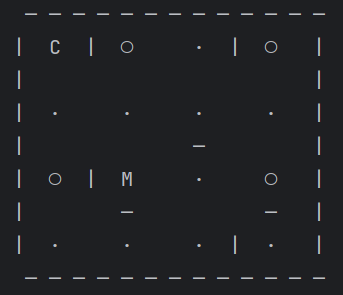
\includegraphics[width=0.5\linewidth]{images/environment.png}
    \caption{A visual representation of the grid environment. The '|'s indicate walls, the 'o's indicate trees, 'C' is the agent, and 'M' is the mouse.}
    \label{fig:environment}
\end{figure}

\begin{figure}
    \centering
    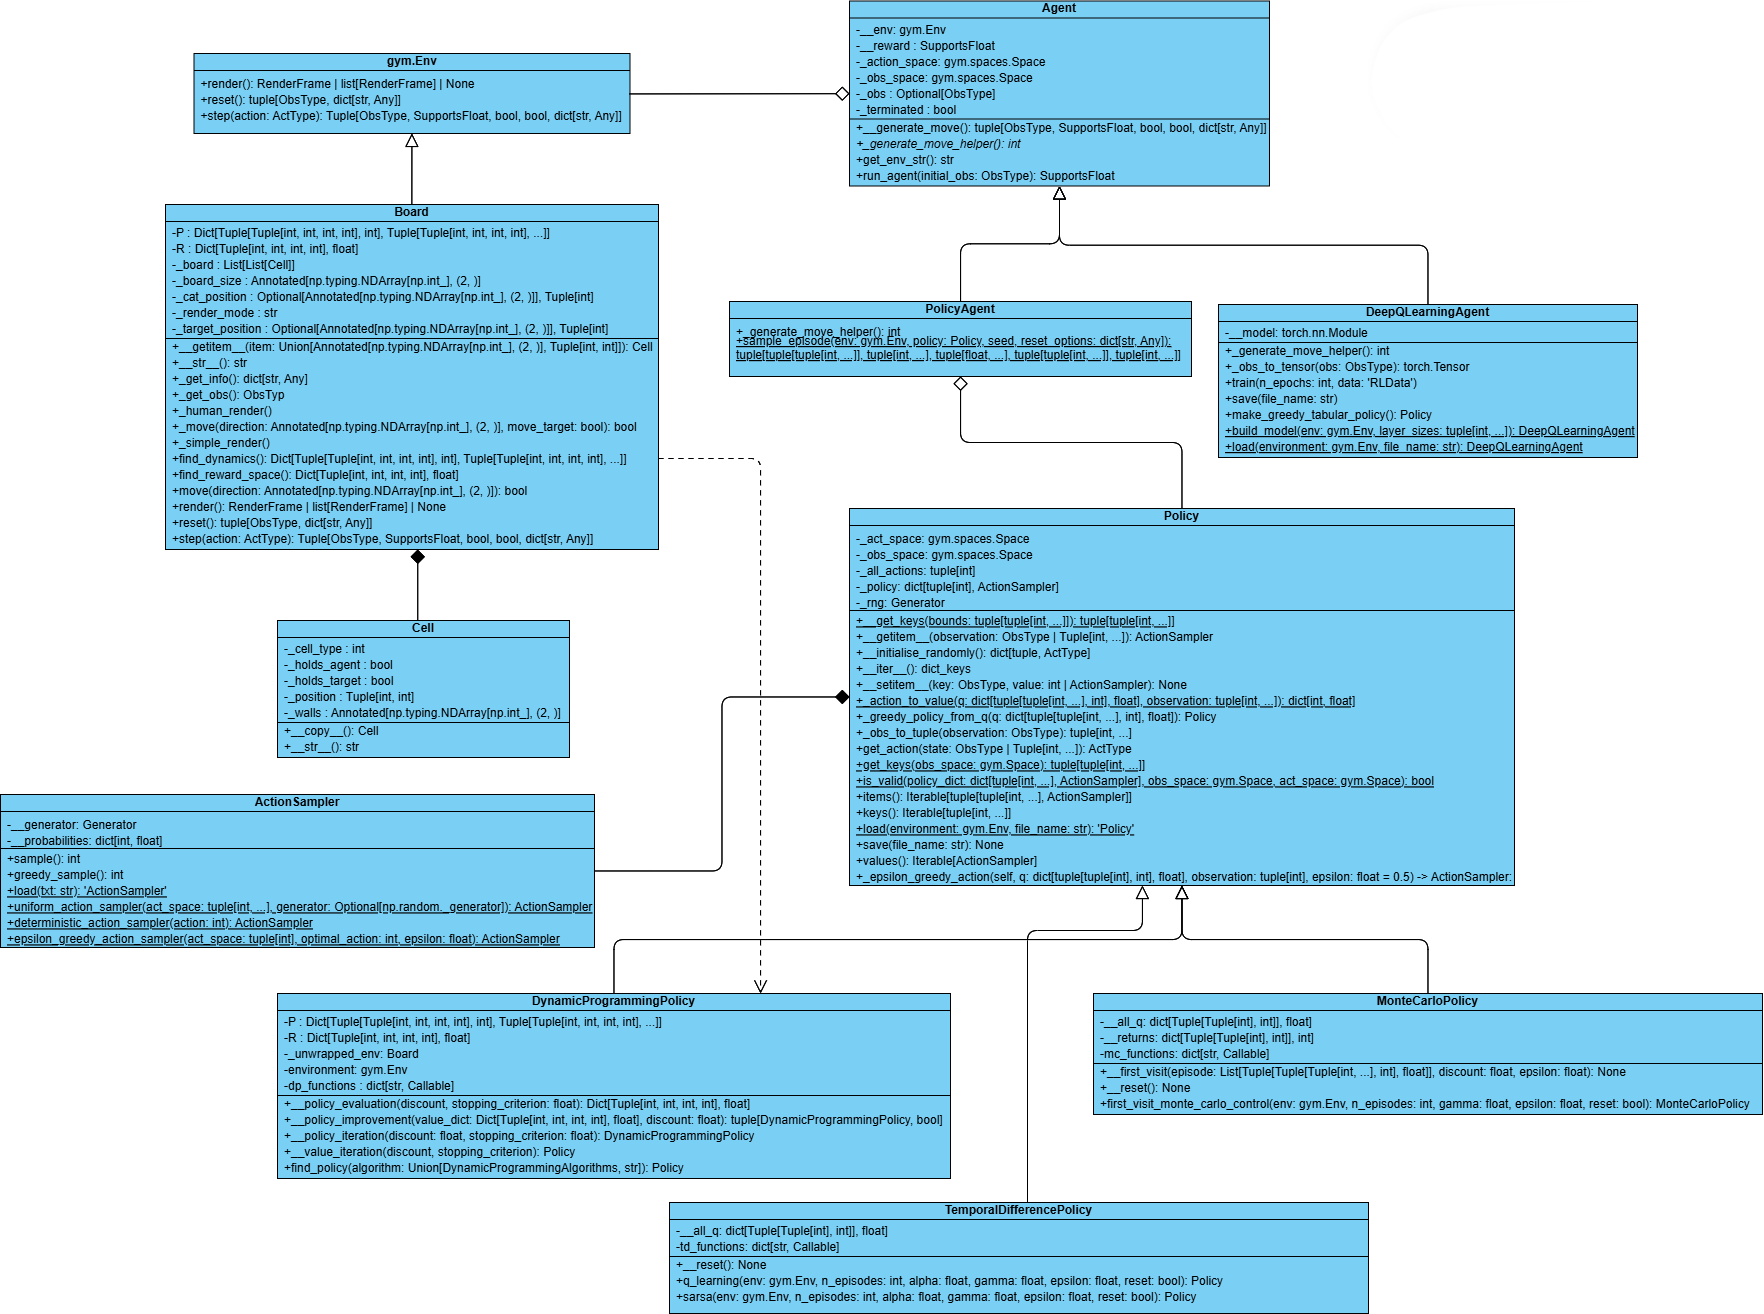
\includegraphics[width=0.99\linewidth]{plots/rl_project_uml.png}
    \caption{Class diagram of the implementation, made with \href{https://online.visual-paradigm.com/}{Visual Paradigm}. Note that the alias \code{gym} was used for the \href{https://gymnasium.farama.org/}{gymnasium} package and the alias \code{np} was used for the \href{https://numpy.org/doc/2.1/index.html}{numpy} package.}
    \label{fig: class diagram}
\end{figure}

\section{Dynamic Programming}
\label{sec: dynamic programming}
The idea behind the first family of algorithms discussed --- Dynamic Programming --- lies in the approach of dividing a large problem (e.g. finding an optimal policy) into smaller sub-problems, like improving a current policy, based on the current estimate of the value function. Solving these smaller subproblems is guaranteed to lead to an optimal solution to the main problem (although it might take infinite iterations).
\\[0.3cm]
For this project, two DP algorithms were implemented and tested: Policy iteration and Value Iteration.

\subsection{Policy Iteration}
The main idea of Policy Iteration is to find an optimal solution through planning. Specifically, the process consists of iteratively evaluating the current policy (through Policy Evaluation) and improving this policy, based on the updates estimate of the value function (through Policy Improvement), until convergence.\\[0.3cm]
Refer to \autoref{fig:policy_iteration_pseudocode} for a full pseudocode.

\subsubsection{Policy Evaluation}
The policy evaluation algorithm relies on the Bellman expectation equations to iteratively update the estimates for the value of each state by considering the values and the rewards of the successor states, weighted by the probability of reaching that state. By iteratively updating the value estimates for each state, the optimal value function can be approximated, omitting the need for complex analytical solutions.
\\[0.3cm]
Note that the convergence to the optimal value function, although guaranteed over infinite iterations, is likely to be computationally expensive. To avoid this issue, a variable delta is defined as the maximal value difference through all the states after the current iteration. When this value becomes low enough, it signifies that the current estimate is close to the true value, and so the algorithm is terminated.

\subsubsection{Policy Improvement}
Policy Improvement algorithm relies on the estimated value function, obtained through Policy Evaluation to determine a new, improved policy though greedily choosing the most promising action. In other words, for every state, the action that is expected to lead to the highest overall reward is chosen for the updated policy.
\begin{figure}[H]
    \centering
    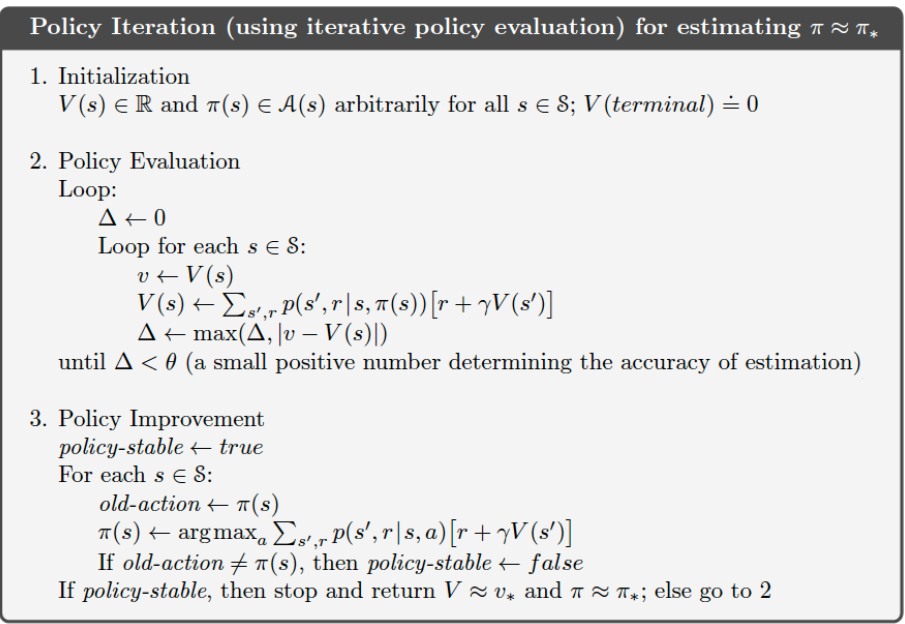
\includegraphics[width=0.5\linewidth]{report_src/images/policy_iteration_pseudocode.png}
    \caption{Policy Iteration pseudocode \parencite[p. 80]{sutton-2018}}
    \label{fig:policy_iteration_pseudocode}
\end{figure}

\subsubsection{Implementation}
This algorithm was implemented as a set of methods in the \code{DynamicProgrammingPolicy} class. This allows the algorithm to update the policy by just modifying itself. The policy itself is stored as a dictionary, mapping each possible observation to the action that is taken. The state-value function is also represented as a dictionary that maps state to value. The policy iteration and policy improvement parts were separated into two methods, the former calling policy evaluation and then policy improvement, until no more changes to the policy are made.

\subsection{Value Iteration}
The principle of optimality states that a policy $\pi$ achieves the optimal value from state s, $v_\pi(s) = v^*(s)$ if and only if from any state $s'$ reachable from s, $\pi$ achieves the optimal value $v_\pi(s') = v^*(s')$. Thus, this theorem directly leads to the value iteration algorithm. With value iteration, the most optimal state value function is computed by iteratively updating the estimate. The algorithm outputs a new approximately optimal policy.
\\[0.3cm]
The process starts by selecting a random value function, over which is iterated using the Bellman equations as an update rule, updating the values for all states. This process gets repeated until convergence to optimal value function, which is guaranteed. Once the optimal value is found, it takes the actions such that the maximum in the Bellman optimality equation is satisfied. For the pseudocode, see \autoref{fig:value_iteration_pseudocode}.

\subsubsection{Implementation}
Value iteration was implemented in code as a method of the \code{DynamicProgrammingPolicy} class. As can be seen in \autoref{fig: class diagram}, this class inherits from \code{Policy}. The algorithm mainly works by storing the state values in a dictionary that has as keys the states and as value the state value. It updates this dictionary using the value obtained by using the Bellman equation on each possible action, picking the value where the action is maximal. It then also updates the action taken in the policy to the new best action.
\\[0.3cm]
Convergence is determined by actively checking the value of \textit{delta} at all states. Once it becomes small enough, the process ends. Since the action taken in each state was already updated during the running of the algorithm, the policy is now approximately optimal.

\begin{figure}[H]
    \centering
    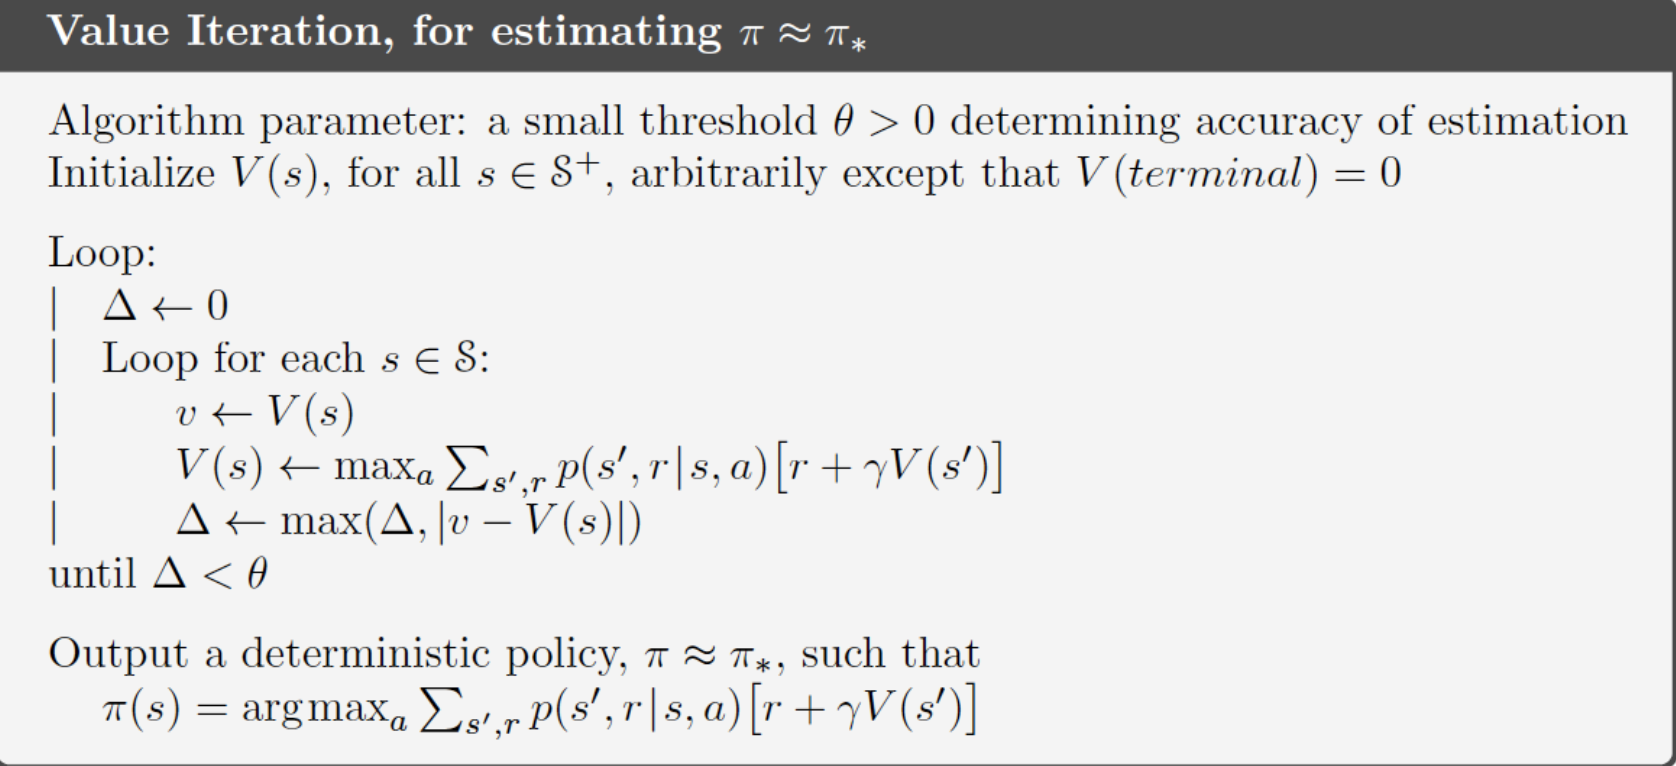
\includegraphics[width=0.5\linewidth]{images/value_iteration.png}
    \caption{Policy Iteration pseudocode \parencite[p. 80]{sutton-2018}}
    \label{fig:value_iteration_pseudocode}
\end{figure}
\section{Monte-Carlo}

\label{sec: monte-carlo}
Monte Carlo (MC) updates the model using data obtained from running simulations of the environment. This allows it to work without assumptions about how the model should work. How MC updates its values differs per method used. In this report, the MC First-Visit on-policy algorithm was used. The pseudocode is given in \autoref{fig: MC psuedocode}.
\begin{figure}[H]
    \centering
    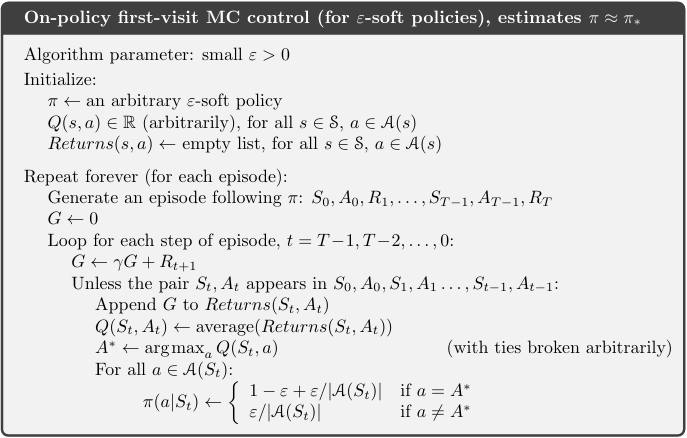
\includegraphics[width=0.5\linewidth]{report_src/images/mc_on_policy_first_visit.png}
    \caption{MC on-policy first-visit pseudocode \parencite[p. 101]{sutton-2018}}
    \label{fig: MC psuedocode}
\end{figure}

\subsection{First-Visit}
After each episode, with First-Visit, the program takes the information learned in an episode and assigns for each state-action pair the gained reward for taking the action plus the discounted total reward for the next pair, see \autoref{eq: first-visit}.
\begin{equation}
    \label{eq: first-visit}
    q(S_t,A_t) = R_{t+1}+\gamma q(S_{t+1},A_{t+1})
\end{equation}
With $S_t$ the state at time $t$, $A_t$ the action taken at time $t$, $R_t$ the reward obtained at time $t$, $\gamma$ the discount, and $q$ the function mapping state and action to their value. This is done for all first encounters of a state-action pair in the episode. Afterwards, the average for each state-action pair is determined over all the values gained for a state-action pair over $n$ episodes.

\subsection{On-Policy}
After each episode, the program looks at all the acquired state-action values. It determines the best action for each state based on which state-action pair has the highest value. To make sure all states and actions are seen by the program, the policy is updated with an $\epsilon$-soft policy, the best action to take will have a higher chance of getting picked but still allow the other actions to be chosen as well. An epsilon soft policy means that the probability of each action given the state is given by \autoref{eq: epsilon greedy}:
\begin{equation}
\label{eq: epsilon greedy}
    \pi (a|s)=\left\{ \begin{array}{rcl}
         1-\varepsilon+\varepsilon/|A(s)|& \mbox{if}& a = \argmax_a Q(s,a)  \\ \varepsilon/|A(s)|
         & \mbox{if} & a \neq \argmax_a Q(s,a)
    \end{array} \right.
\end{equation}
This way of updating the policy guarantees that the new policy is better than the one before but it cannot guarantee an optimal policy.

\subsection{Implementation}
The algorithm was implemented as a method of the \code{MonteCarloPolicy} class (for class structure, see \autoref{fig: class diagram}). The code first samples an episode using itself as a policy, and then updates its internal $Q$ function, which is a dictionary mapping state-action to a reward, based on the episode returns. The policy then updates itself by creating an $\epsilon$-greedy \code{ActionSampler} on the optimal action, assigning it to the current state. Note that $\epsilon$ does not decay, so the policy will always stay $\epsilon$-soft.

\section{Temporal Difference}
\label{sec: temporal difference}
Temporal Difference (TD) Learning algorithms are another set of algorithms that learn the environment from experience rather than by computing the optimal policy based on a model. It achieves this by learning the optimal state-action value function $q^*(s, a)$ by sampling many episodes. While this is similar to Monte-Carlo methods described in \autoref{sec: monte-carlo}, Temporal Difference learning does not use the full return computed at the end of the episode; rather it uses bootstrapping to allow it to update the $Q(s, a)$ after each step taken in the episode. This enables it to be used in environments without terminal states. In comparison to Monte-Carlo, TD algorithms generally have higher bias but lower variance. 
\\[0.3cm]
Two main variants of Temporal Difference learning are discussed in this report: SARSA, an on-policy control algorithm, discussed in \autoref{subsec: sarsa}, and Q-learning, an off-policy control algorithm, discussed in \autoref{subsec: q-learning}. 

\subsection{SARSA}
\label{subsec: sarsa}
SARSA is an on-policy temporal difference learning control algorithm. SARSA is short for 'State, Action, Reward, State, Action', which refers to how the state-action value function is updated at each time step. The goal of the algorithm is to approximate $Q(s,a) \approx q^*(s,a)$. This is done by sampling many episodes, and for each step of the episode, updating the value function using the following update rule:
\begin{equation}
    \label{eq: sarsa}
    Q(S,A) := Q(S,A) + \alpha(R + \gamma Q(S', A') - Q(S, A))
\end{equation}
Note that $\alpha$ is the learning rate, $\gamma$ is the discount factor, $S$ is the current state, $S'$ is the next state, which is reached after taking action $A$. Finally, $A'$ is the action taken from state $S'$. This action is generated by acting $\epsilon$-greedy on $Q$ for the given state. 
\\[0.3cm]
The algorithm works by first initalising for all state, action pairs, $Q(s,a) = 0$. It will then repeat the following over a prespecified number of episodes. It first picks an action taken from the starting state of the episode, after which it will first take the determined action, get the new state $S'$, use this new state together by acting $\epsilon$-greedy on the value function to get a new action $A'$, after which \autoref{eq: sarsa} is used to update the state-action value function. This is repeated until the episode is finished.
\\[0.3cm]
Compared to Q-Learning, SARSA generally chooses a safer path during training, which makes it more likely to converge on an optimal policy, while it does cause it to need more steps than Q-Learning.

\subsubsection*{Implementation}
This algorithm was implemented as a method of the \code{TemporalDifferencePolicy} class (for class structure, see \autoref{fig: class diagram}). The code learns over $n$ episodes, each episode deciding its actions $\epsilon$-greedy, updating its state-action value function $Q$ along the way, which is represented by a dictionary mapping state-action pairs to their value. When finished, it computes a new policy by acting greedily on the value function. This policy is then returned. Note that usually, the policy derived from $Q$ is $\epsilon$-greedy. However, this implementation acts greedily instead in the final policy, since it is assumed to have arrived at an approximately optimal policy. 

\subsection{Q-Learning}
\label{subsec: q-learning}
Q-learning is an off-policy algorithm, meaning that it learns the value of the optimal policy independently of the action values \parencite{off-policy-q-learning}. The algorithm is very similar to the value iteration one. While value iteration tries to find the optimal value, q-learning aim at estimating the optimal Q-function. Same as for value iteration, convergence is guaranteed for sufficient experience. The goal of Q-learning is to determine the optimal action based on the current state. The update rule of Q-learning is as follows:
\begin{equation}
    \label{eq: sarsa}
    Q(S,A) := Q(S,A) + \alpha(R + \gamma \max_a Q(S', A') - Q(S, A))
\end{equation}
\\[0.3cm]
The algorithm works by initializing a Q-table, which stores the action-values sets. The process continues by selecting and performing an action, after which the reward is measured and the the Q-table gets updated. The process ends when a terminal state \textit{s} is reached.
\\[0.3cm]
Of great importance is that Q-learning has maximization bias. A solution to this is Double Q-learning, which uses two Q-functions but does not get updated at the same time.

\subsubsection*{Implementation}
The implementation of Q-Learning is extremely similar to that of SARSA. The main difference in the implementation is that the action chosen to update the $Q$ dictionary is a greedy action on $Q$, instead of the actual action taken. Other than that, there are no differences with SARSA.

\section{Comparison and Discussion}
\label{sec: comparison and discussion}
As can be seen from the plots below, the results derived from Policy Iteration and Value Iteration are strikingly similar. This indicates that both algorithms likely converged to an optimal policy. Both policies seem to mostly reach the terminal state after taking 3-6 steps with the highest average reward being at the fifth time stamp. This indicates that most episodes end quickly, suggesting a great performance of the determined policy.

\begin{figure}[H]
    \centering
    \begin{subfigure}[t]{0.48\linewidth}
        \centering
        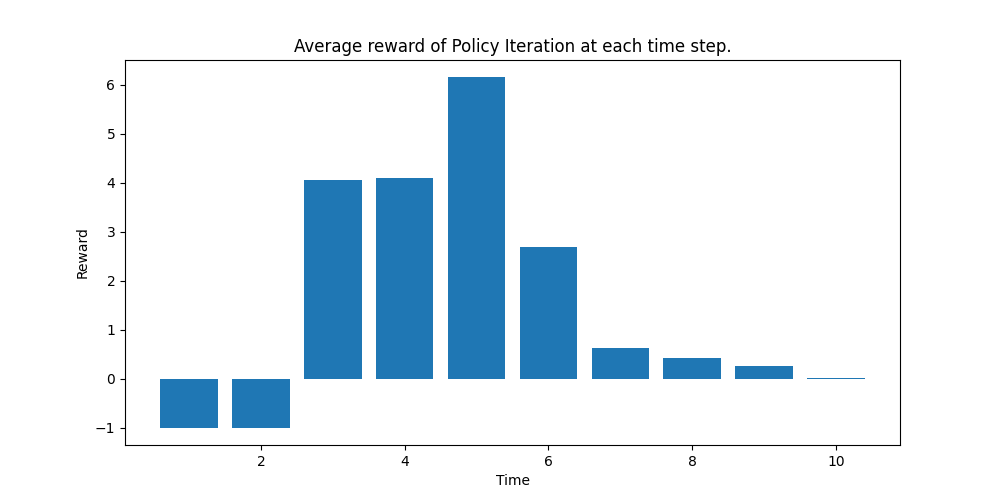
\includegraphics[width=\linewidth]{plots/r_over_time/policy_iteration_r_over_time.png}
        \caption{Policy Iteration}
        \label{fig:policy_iteration_r_over_time}
    \end{subfigure}
    \hfill
    \begin{subfigure}[t]{0.48\linewidth}
        \centering
        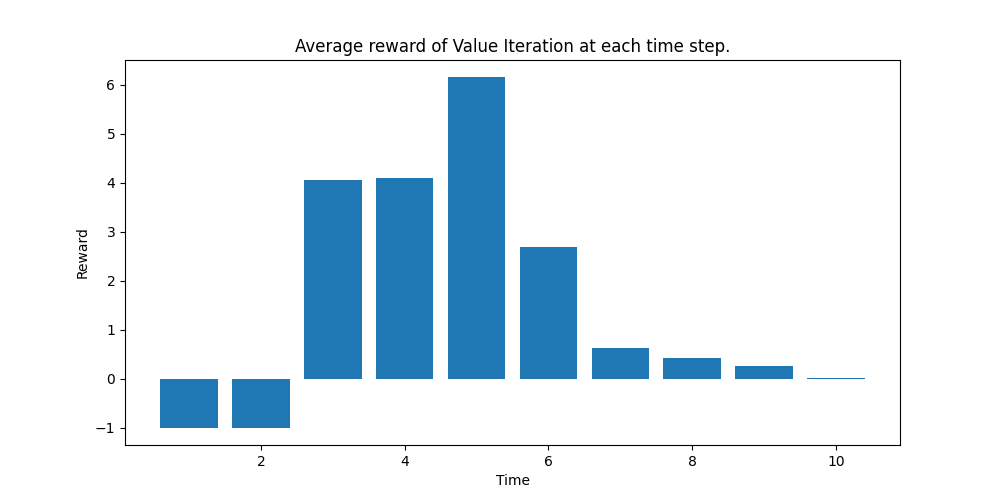
\includegraphics[width=\linewidth]{plots/r_over_time/value_iteration_r_over_time.png}
        \caption{Value Iteration}
        \label{fig:value_iterations_r_over_time}
    \end{subfigure}
    \caption{Average reward at each time step for both Policy Iteration and Value Iteration.}
    \label{fig:DP_reward_comparison}
\end{figure}

\noindent This interpretation is further supported by the plots of the probability density functions of the returns derived from both policies. The plots are once again (almost) identical and indicate that the highest reward likelihood for these policies is around 16, aligning with the 3-6 steps with the rewards of -1 from before.

\begin{figure}[H]
    \centering
    \begin{subfigure}[t]{0.48\linewidth}
        \centering
        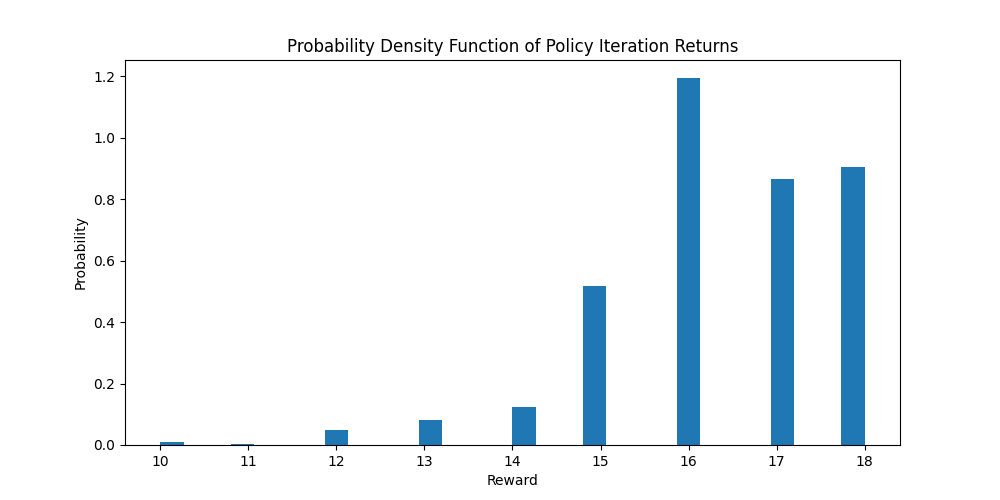
\includegraphics[width=\linewidth]{plots/return_probability/policy_iteration_return_probability.png}
        \caption{Policy Iteration}
        \label{fig:policy_iteration_return_probability}
    \end{subfigure}
    \hfill
    \begin{subfigure}[t]{0.48\linewidth}
        \centering
        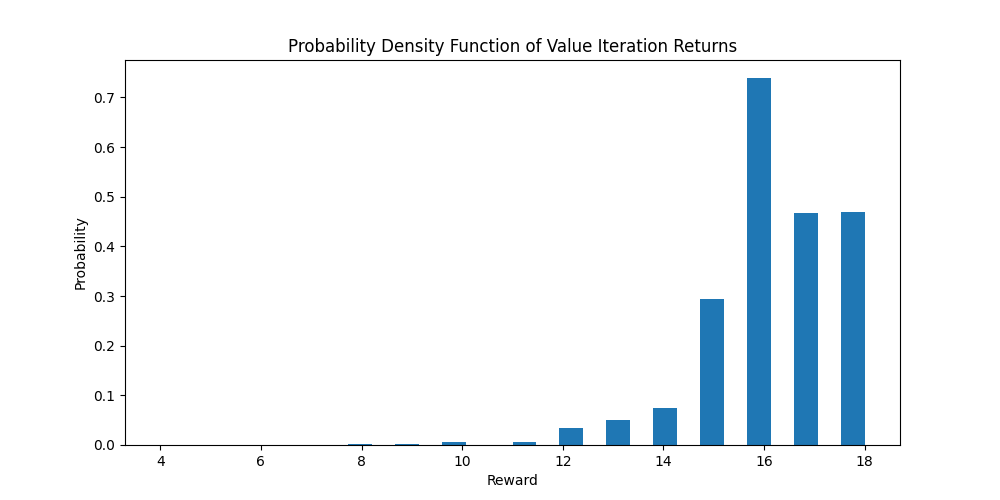
\includegraphics[width=\linewidth]{plots/return_probability/value_iteration_return_probability.png}
        \caption{Value Iteration}
        \label{fig:value_iterations_return_probability}
    \end{subfigure}
    \caption{Return probability distributions for Policy Iteration and Value Iteration.}
    \label{fig:DP_return_probability_comparison}
\end{figure}

\noindent The Monte Carlo algorithm, on the other hand, failed to arrive at an optimal policy over 100 steps (more steps did not help, as can be seen in \autoref{fig: comparison mc, ql, sarsa}). The plots from \autoref{fig:monte_carlo_r_over_time_and_return_probability} indicate a lower average reward for all time steps, compared to the DP algorithms from earlier. Furthermore, the probability density function suggests that the policy, derived from First Visit Epsilon Greedy Monte Carlo, results in a much higher likelihood of returning a negative reward than any of the DP policies. This can be explained by the fact that Dynamic Programming algorithms have a full context of the environment and use planning internally, while Monte Carlo needs to rely on the limited information obtained through the interaction with the environment.

\begin{figure}[H]
    \centering
    \begin{subfigure}[t]{0.47\linewidth}
        \centering
        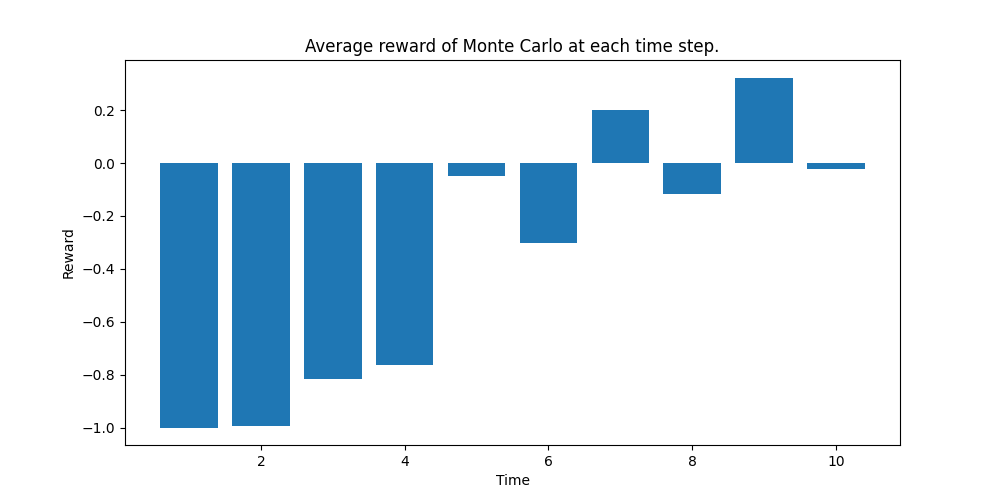
\includegraphics[height=4.2cm]{plots/r_over_time/monte_carlo_r_over_time.png}
        \caption{Average reward at each time step}
        \label{fig:monte_carlo_r_over_time}
    \end{subfigure}
    \begin{subfigure}[t]{0.47\linewidth}
        \centering
        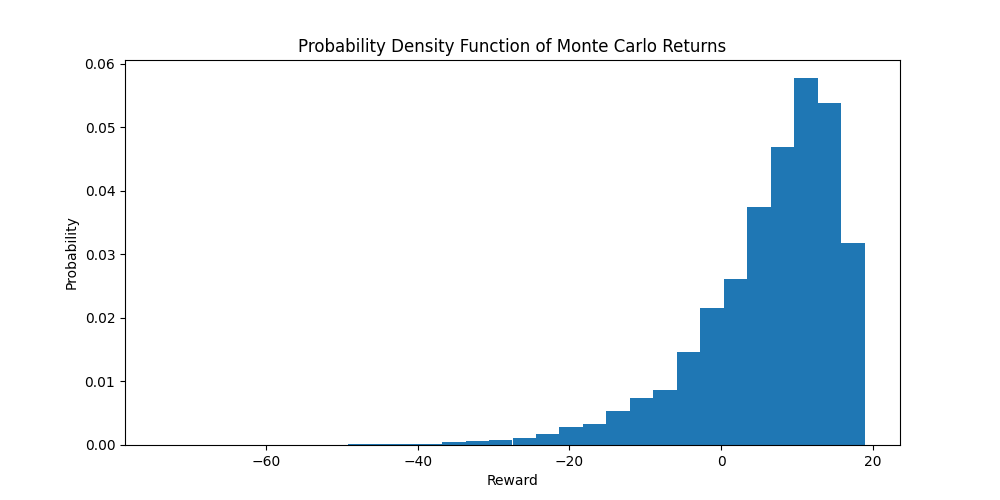
\includegraphics[height=4.2cm]{plots/return_probability/monte_carlo_return_probability.png}
        \caption{Return probability distributions}
        \label{fig:monte_carlo_return_probability}
    \end{subfigure}
    \caption{Average reward over time and the Return probability distribution for Monte Carlo.}
    \label{fig:monte_carlo_r_over_time_and_return_probability}
\end{figure}

\noindent As for the Temporal Difference algorithms (see \autoref{fig:sarsa_qlearning_comparison}), both SARSA and Q-Learning seem to perform quite similarly, with SARSA displaying a slightly better performance. Similar to results from the DP algorithms, it can be seen that the first two steps yield a negative reward, though unlike Q-Learning, SARSA learned to obtain significant positive reward on the third step. The return probability distributions indicate a low chance of receiving a negative total reward, displaying a significantly higher performance compared to MC.

\begin{figure}[H]
    \centering
    % First row: Average rewards
    \begin{subfigure}[t]{0.47\linewidth}
        \centering
        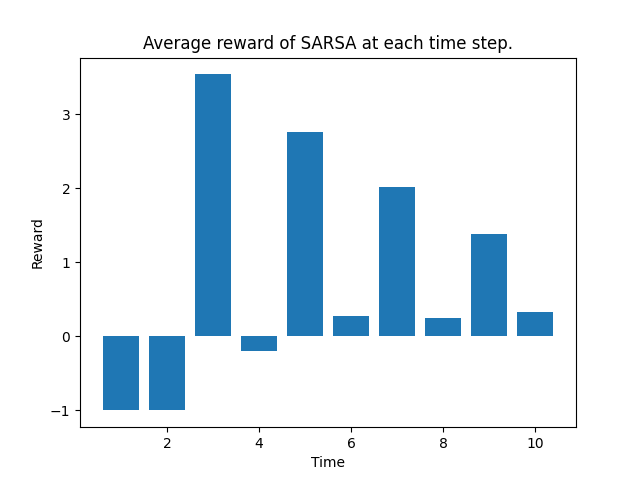
\includegraphics[height=4.2cm]{plots/r_over_time/sarsa_r_over_time.png}
        \caption{SARSA: Average reward at each time step}
        \label{fig:sarsa_r_over_time}
    \end{subfigure}
    \hspace{0.03\linewidth}
    \begin{subfigure}[t]{0.47\linewidth}
        \centering
        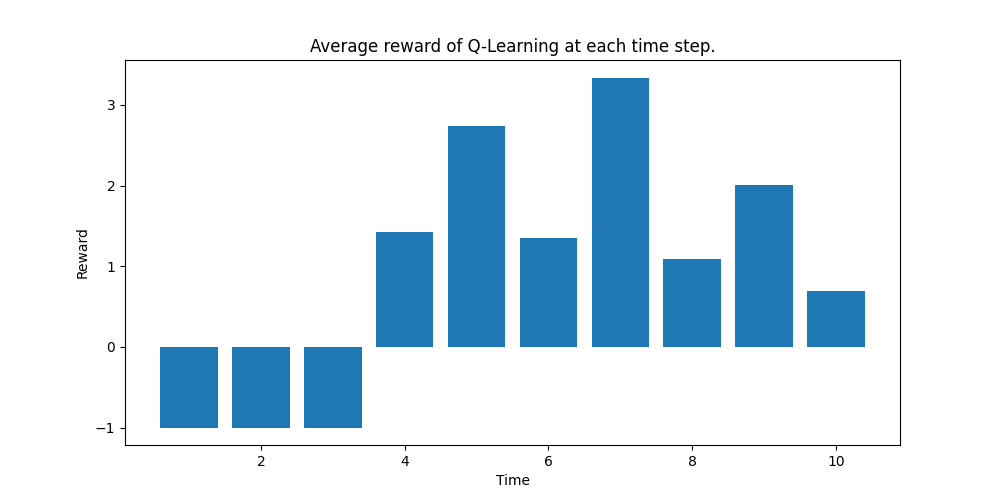
\includegraphics[height=4.2cm]{plots/r_over_time/q_learning_r_over_time.png}
        \caption{Q-Learning: Average reward at each time step}
        \label{fig:qlearning_r_over_time}
    \end{subfigure}

    \vspace{0.5cm} % Add vertical space between rows

    % Second row: Return distributions
    \begin{subfigure}[t]{0.47\linewidth}
        \centering
        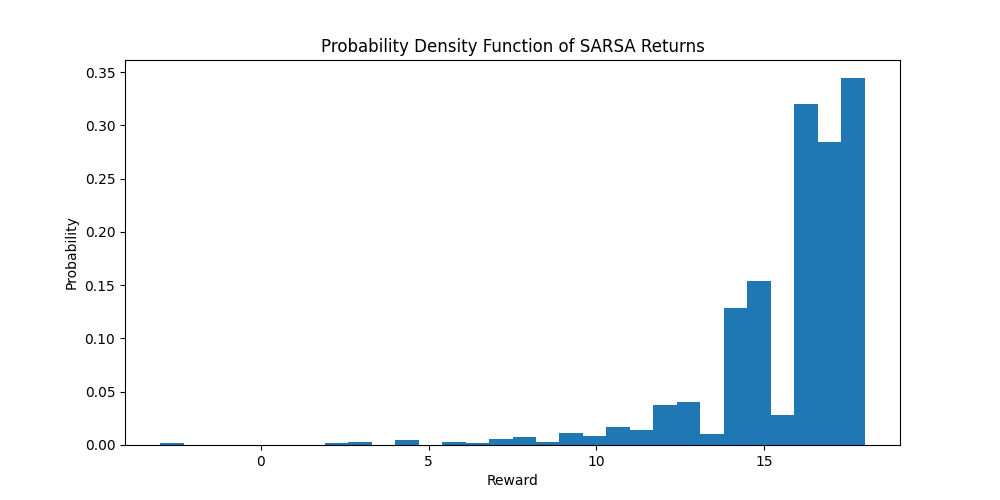
\includegraphics[height=4.2cm]{plots/return_probability/sarsa_return_probability.png}
        \caption{SARSA: Return probability distribution}
        \label{fig:sarsa_return_probability}
    \end{subfigure}
    \hspace{0.03\linewidth}
    \begin{subfigure}[t]{0.47\linewidth}
        \centering
        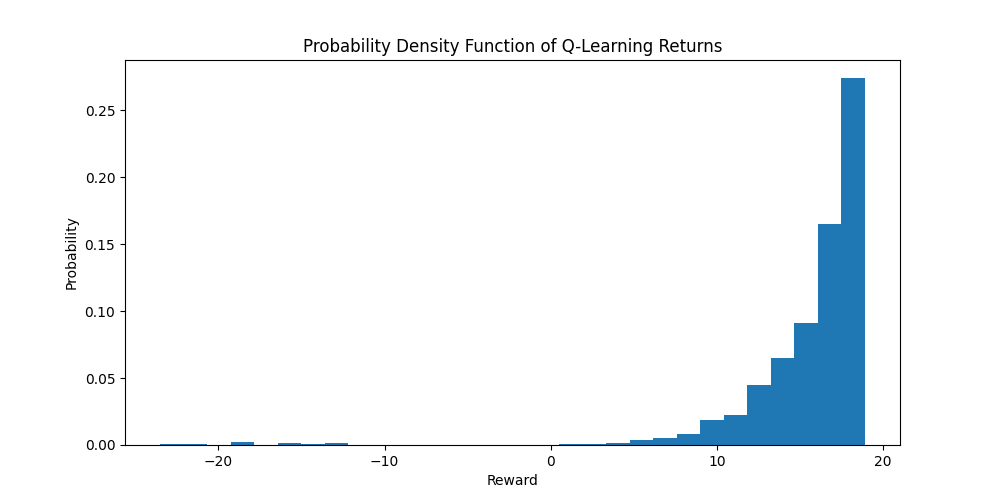
\includegraphics[height=4.2cm]{plots/return_probability/q_learning_return_probability.png}
        \caption{Q-Learning: Return probability distribution}
        \label{fig:qlearning_return_probability}
    \end{subfigure}

    \caption{Comparison of SARSA and Q-Learning. Top row (a, b): Average reward over time. Bottom row (c, d): Return probability distributions.}
    \label{fig:sarsa_qlearning_comparison}
\end{figure}

\noindent When comparing the learning behaviour of First-Visit Monte Carlo, Q-Learning, and SARSA (see \autoref{fig: comparison mc, ql, sarsa}), it can be seen that both SARSA and Q-Learning stabilise quite quickly at the same average reward obtained, after about 50 learning steps. Monte-Carlo also stabilises at this point, although it is less stable and has a lower average value. 

\begin{figure}[H]
    \centering
    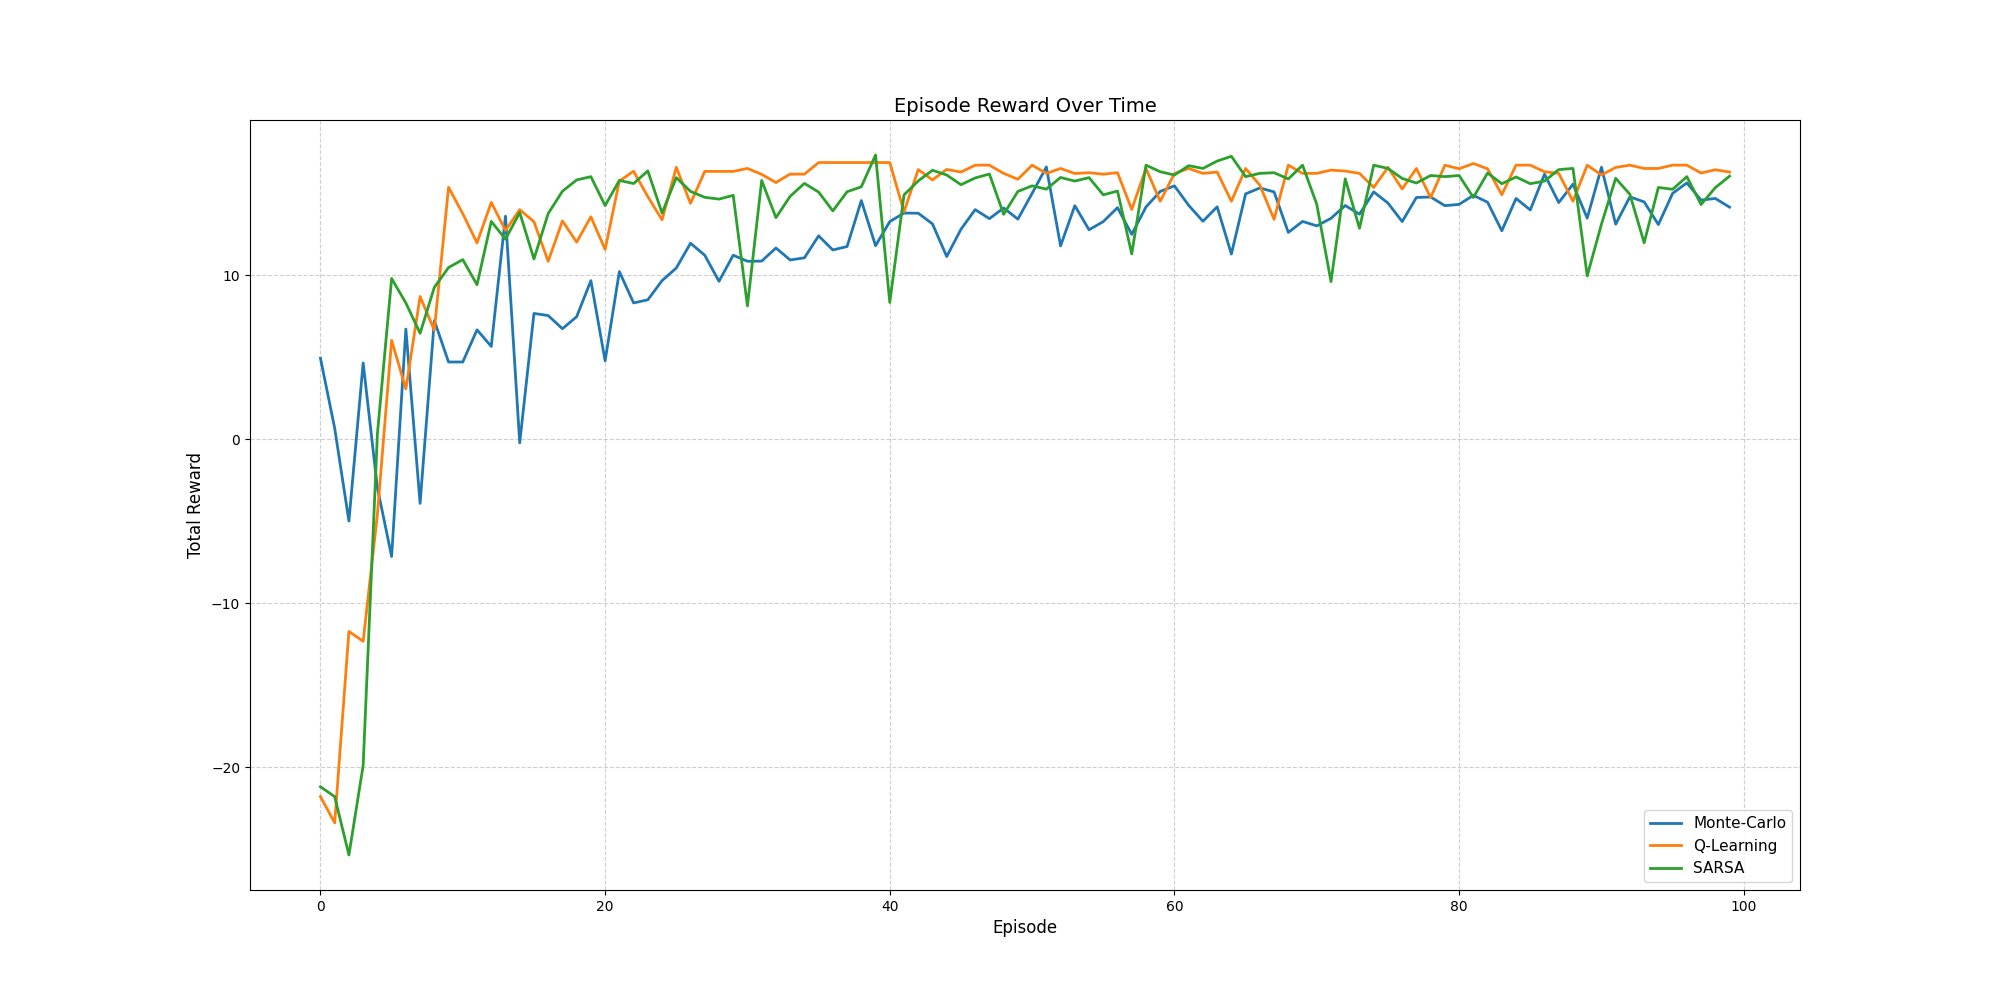
\includegraphics[width=0.7\linewidth]{plots/comparison/comparison_plot_final.png}
    \caption{Comparison of the average reward evolution over the course of learning of First-Visit Monte Carlo, Q-Learning, and SARSA}
    \label{fig: comparison mc, ql, sarsa}
\end{figure}


\section{Conclusion}
In this report, some common algorithms used in Reinforcement Learning (RL) were discussed. These algorithms include Policy Iteration, Value Iteration, First-Visit Epsilon-Greedy Monte Carlo, SARSA, and Q-learning. Having analysed data from all the algorithms (see \autoref{fig:total_return_ocmparison}), it was found that Dynamic Programming algorithms (Policy Iteration and Value Iteration) arrived at the best-performing optimal policy. This result indicates that for the cases where the environment is known (or can be easily learned), DP is a great choice.
\\[0.3cm]
SARSA and Q-Learning fall shortly behind, with SARSA slightly outperforming Q-Learning. Those algorithms did not have any direct knowledge of the environment, and yet were able to arrive at a great policy after seeing 100 episodes for the environment used in this report. Q-Learning 'prefers' to act more risky, resulting in a lower average reward.
\\[0.3cm]
First-Visit Epsilon-Greedy Monte Carlo yielded the worst results of all the policies. The results clearly indicate that it performs significantly better than the random policy, indicating that it did learn from the environment. Yet, First Visit MC only learns from the first instance of the state-action pair in an episode, making the convergence slower.

\begin{figure}[H]
    \centering
    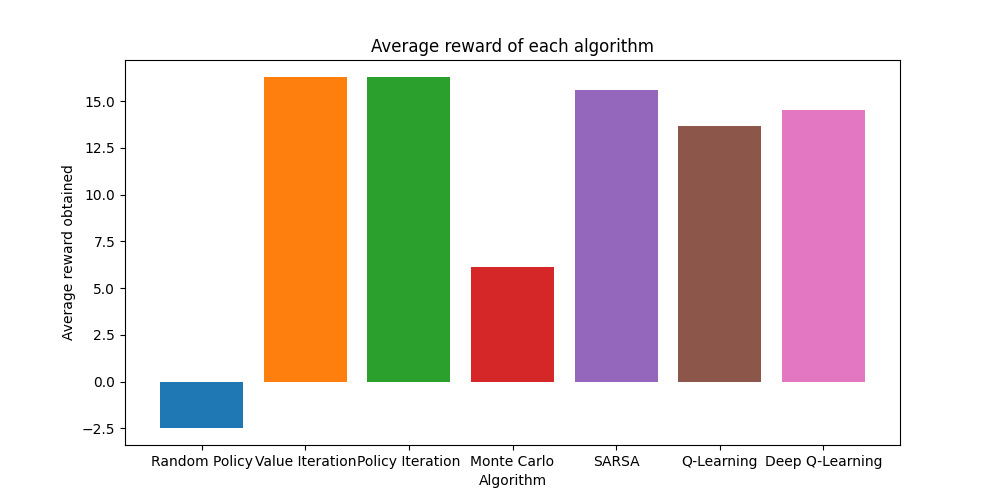
\includegraphics[width=0.5\linewidth]{plots/comparison/total_return_comparison.png}
    \caption{Comparison of the average (over 1000 episodes) final return achieved by each algorithm.}
    \label{fig:total_return_ocmparison}
\end{figure}


\printbibliography[title={References}]

\begin{appendices}

\section{Deep Q-Learning}
\label{app: deep q-learning}
As an additional exercise, Deep Q-learning (DQL) was implemented. In contrast to the algorithms discussed in the main report, Deep Q-Learning is not tabular, meaning that it does not compute a lookup table for every single state. This is mainly useful when dealing with environments that have an extremely large observation space since it would be impossible to use tabular methods for these types of environments since training would take too long while likely also taking too much space to store all information.

\subsection{Theoretical Deep Q-Learning}
Deep Q-Learning uses a neural network to circumvent the need for lookup tables. At the output layer, this neural network needs to have one neuron for each possible action. The output value of a single neuron in the output layer represents the value of this action in the given state. From these output values, the optimal action can for instance be selected greedily by picking the action with the largest value (softmax could also be used, picking each action at the probability specified by softmax). 
\\[0.3cm]
The input layer of the neural network needs to be able to take an observation from the environment. In the case of the environment used in this report, there are 4 input neurons, the first two representing the agent position, the latter two representing the target position. However, for an agent that would for example observe the world with a camera, the flattened image could be used as input for the network.
\\[0.3cm]
In order to train a neural network, gradient descent (GD) is used. To allow GD to be used, there needs to be a loss function. According to \textcite{lecture6}, the loss for DQL can be computed using \autoref{eq: dql loss}:
\begin{equation}
    \label{eq: dql loss}
    L_t(\mathbf{w}_t) = \mathbb{E}\left[\left(R_{t+1} + \gamma\max_{a'}(S_{t+1}, a';\mathbf{w}_{t-1}) - Q(S_t, A_t;\mathbf{w}_t)\right)^2\right]
\end{equation}
With $t$ the time, $R_t$ the reward at time $t$, $S_t$ the state at time t, $A_t$ the action taken at time $t$, $\mathbf{w}_t$ the weights of the model at time $t$, $a'$ the set of actions that can be taken, and $Q$ the model, that gives the value of a state and action computed using the weights of the model.

\subsection{Practical Deep Q-Learning}
The basic implementation of DQL is fairly simple. Two models are maintained, the previous model and the current one. The model is trained by looping over many episodes, at each step in the episode, obtaining the reward and next state, then taking an action using some policy, and using this information to compute the loss using \autoref{eq: dql loss}. 
\\[0.3cm]
There are, however, some issues with this implementation of DQL. Firstly, the target is determined by the previous model. Since this model is constantly updating, the algorithm is chasing a moving target, which can lead to algorithm instability \parencite{lecture6}. To solve this issue, instead of moving the target after every step, the target is moved after $n$ steps. This somewhat improves model stability.
\\[0.3cm]
This improvement to the base algorithm was still not enough to make DQL work. This was caused by that the model trains on each episode only once, and that all data it trains on is sequential, making the model constantly need to adapt to the current episode. To circumvent this issue, experience replay was used. Many episodes were sampled, for each episode storing a tuple of $(S, A, R, S', T)$ (with $T$ indicating if $S'$ is terminal). This data was then randomly shuffled and trained on using mini-batch gradient descent over a few epochs. This allowed the model to converge on a good policy.
\\[0.3cm]
The final model trained was trained on 100000 randomly sampled episodes, training on it in 10 epochs. A learning rate of 0.01 was used, a discount of 0.9 was used, and the batch size was set to 1024. The model was set to reset the target model every 10 batches. The final model receives the average rewards plotted in \autoref{fig: dql over time} at every time step when the agent starts in the top left corner of the environment and the agent starts in the bottom right. Furthermore, the probability distribution of the return was plotted in \autoref{fig: dql return probability}. Note that there were a few extremely bad episodes in there, but in general, the model performs quite well, although not as well as SARSA and Q-Learning. Furthermore, the model does take quite some time to train, and sampling all the data required takes even longer.
\\[0.3cm]
In conclusion, the Deep Q-Learning algorithm discussed in this report seems to be able to somewhat approximate an optimal policy, and in cases where tabular algorithms are not possible, DQL could be a good alternative. However, when tabular solutions are feasible, it seems to be more efficient to just use a tabular algorithm such as Q-Learning instead.

\begin{figure}
    \centering
    \begin{subfigure}[t]{0.47\linewidth}
        \centering
        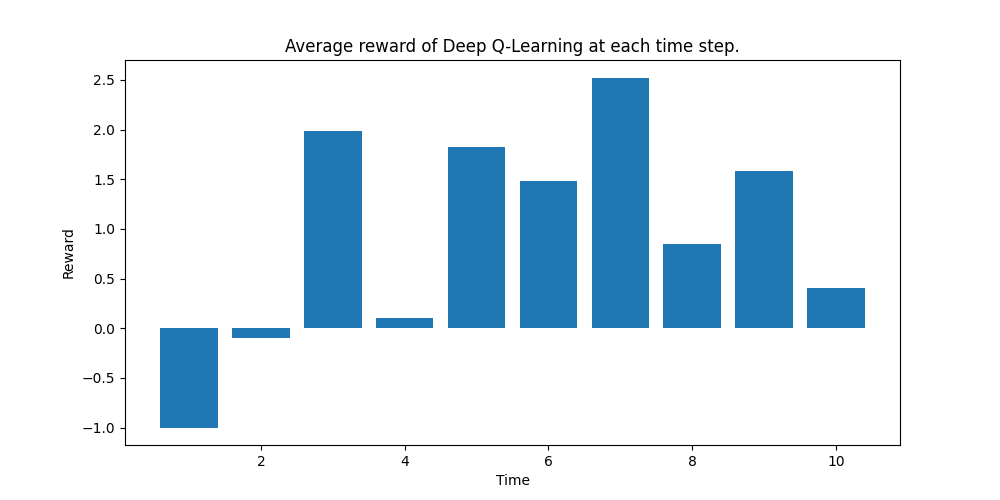
\includegraphics[width=1\linewidth]{plots/r_over_time/deep_q_learning_r_over_time.png}
        \caption{The average reward received by Deep Q-Learning at each time step.}
        \label{fig: dql over time}
    \end{subfigure}
    \begin{subfigure}[t]{0.47\linewidth}
        \centering
        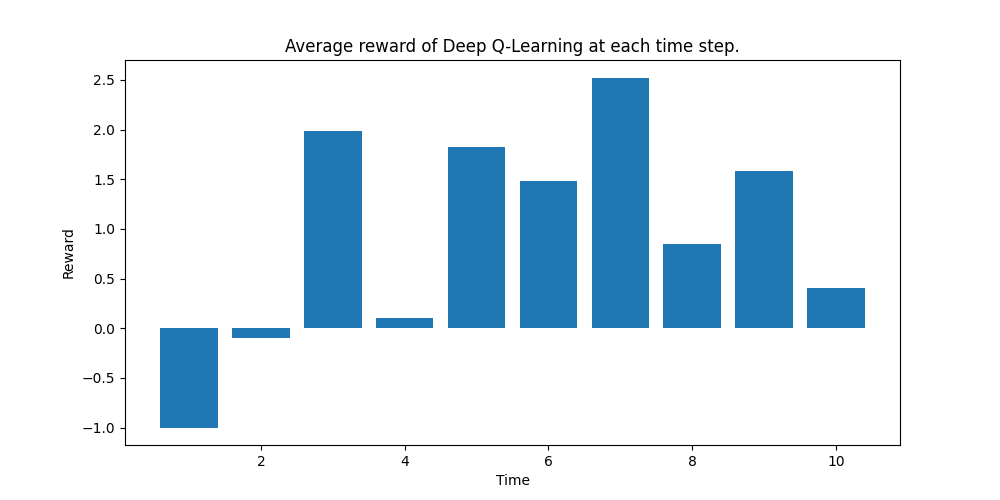
\includegraphics[width=1\linewidth]{plots/r_over_time/deep_q_learning_r_over_time.png}
        \caption{Return probability distributions}
        \label{fig: dql return probability}
    \end{subfigure}
    \caption{Average reward over time and the Return probability distribution for Deep Q-Learning}
    \label{fig: dqlstuff}
\end{figure}

\end{appendices}


\end{document}
